\label{sec:intro}

The cooperation of agents can expand the capability of the unmanned system, and the multi-agent intelligent system is a promising research field.
Multi-Robot Exploration (MR-Exploration)  ~\cite{corah2019communication} provides location and map for each robot, and is the basic task for many multi-robot applications, such as multi-robot navigation  ~\cite{tanner2005towards} and multi-robot rescue  ~\cite{baxter2007multi}.


\begin{figure}[t]
    \centering
    % \vspace{-0.1cm} 
    % \setlength{\abovecaptionskip}{0cm} 
    % \setlength{\belowcaptionskip}{-0.4cm} 
	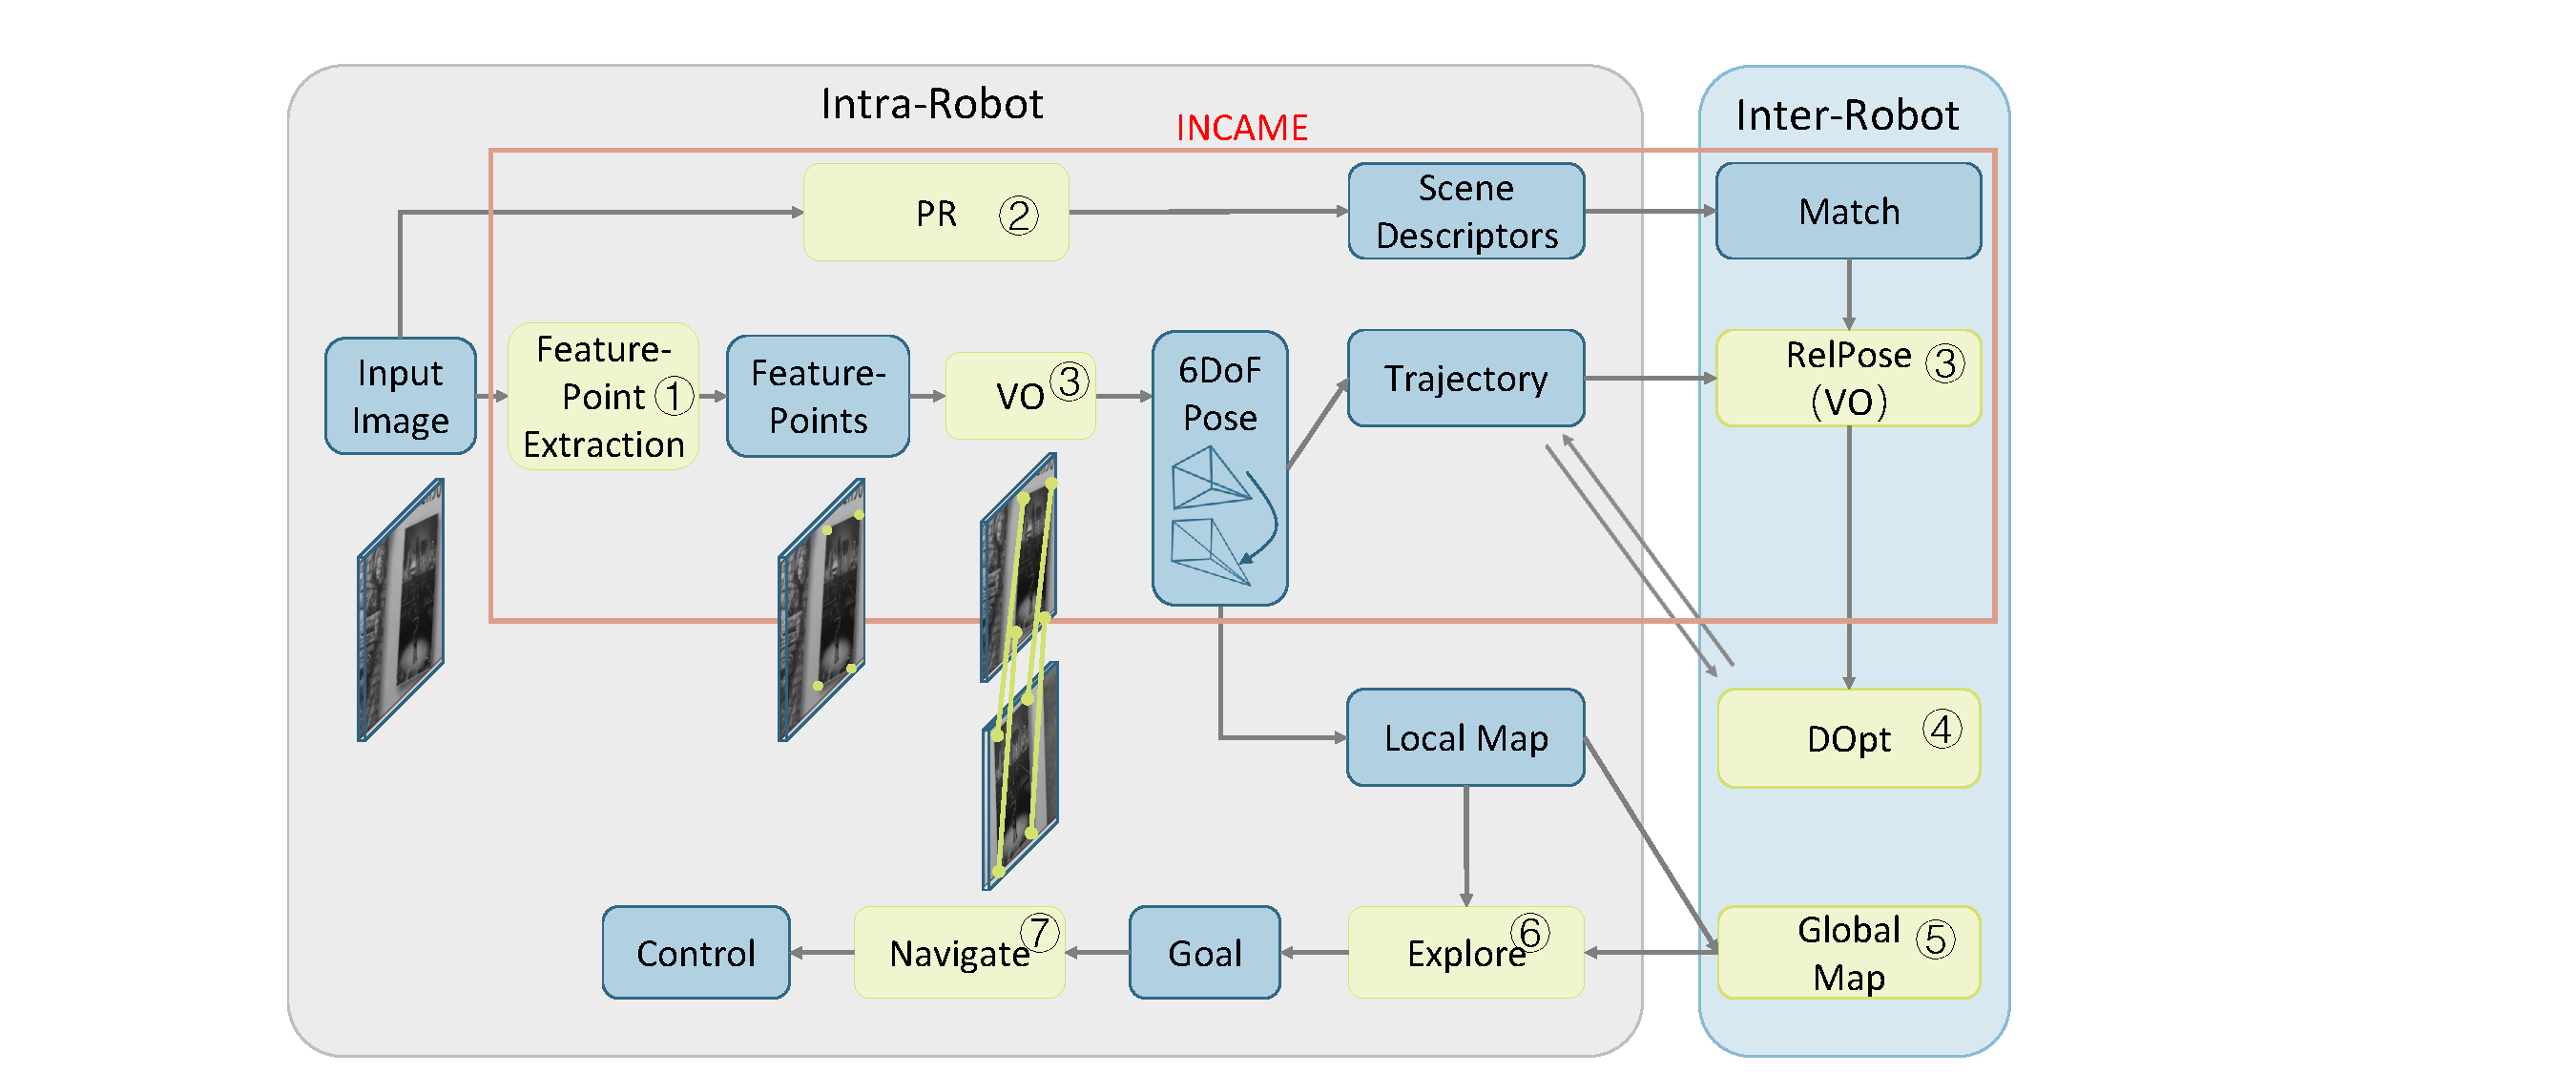
\includegraphics[width=0.99\linewidth]{fig/maexp.pdf}
     \caption{
        The components in MR-Exploration.  Each frame is required to execute \textcircled{1}\textcircled{3} with low latency. \textcircled{2} runs on some keyframes. INCAME implements \textcircled{1} \textcircled{2} on the CNN accelerator, and optimizes the scheduling among \textcircled{1} \textcircled{2} \textcircled{3}.
    }
%     \caption{
%         The components in MR-Exploration. \textcircled{1}\textcircled{3} are basic for a single robot, should be execute every frame. \textcircled{2} generates representation code for some keyframes. \textcircled{4}\textcircled{5} are only executed when representation codes are matched across robots and they are latency tolerant.  \textcircled{6}\textcircled{7} are used for decision and navigation, also latency tolerant.
%     }
	\label{fig:maexp}
\end{figure}

The  MR-Exploration system  ~\cite{corah2019communication, cieslewski2018data} consists of several robots, and each robot executes the system illustrated in \Cref{fig:maexp}. Each input frame is fed to the Feature-point Extraction (FE, \textcircled{1}) module for Visual Odometry (VO). 
Some input frames, called keyframes, are fed to the Place Recognition (PR, \textcircled{2}) module.
PR module generates the compact image representation, which produces the candidate place recognition matches between different robots. 
The Visual Odometry (VO) (\textcircled{3}) matches the feature-points of two adjacent frames to produce the 6 Degrees of Freedom (6-DoF) poses. 
\textcolor{blue}{
Although the VO outputs the 6-DoF poses, which is represents the pose in 3D space, we build the 2D map only using several lines of the camera. 
By projecting the 3D poses into 2D map to navigate the robots, we significantly reduce the computational cost of building maps.
Furthermore, each 2D map is aligned to a key-frame \cite{ho2018virtual,sodhi2019online}.
Through optimizing the keyframe trajectory poses, the map can be synchronously optimized and merged.
}
% Based on the 6-DoF poses,  map and the trajectory can be used for location.
The relative pose (RelPose) module does the same operation as VO(\textcircled{3}) and establishes relative poses between the candidate place matches of different robots. 
The decentralized optimization module (DOpt, \textcircled{4}) optimizes the intra-robot relative pose measurements from VO and the inter-robot relative pose measurements from RelPose. 
\textcolor{blue}{
We use the Pose Graph Optimization (PGO) \cite{Choudhary:2017e66} to do DOpt. 
PGO only optimizes the keyframe trajectory pose without optimizing the keypoints. 
Because the number of keyframe is far less than the number of feature-points, PGO is much faster than Bundle Adjustment (BA) algorithm \cite{wu2011multicore}, which not only optimize the trajectory but also the feature-points.
}
The global map generation module (\textcircled{5}) merges the maps. The exploration module (\textcircled{6}) decides an unexplored goal point for each robot to move based on the merged map and the estimated location. The navigation module (\textcircled{7}) guides each robot to the goal point, including path planning and obstacle avoidance.

\textcolor{blue}{
With the help of 2D maps (\textcircled{5}) and fast PGO (\textcircled{4}), we deploy map merging and optimization on the embedded CPU. 
PR (\textcircled{2}), feature-point extraction (\textcircled{1}), and VO (\textcircled{3}) become the most computational intensive modules. We optimize the scheduling these components across the CPU side (processing system, PS) and FPGA side (programmable logic, PL), on Xilinx MPSoC  ~\cite{MPSoC}.
}



% \Cref{fig:maexp} illustrates the computation modules in MR-Exploration.
% Feature-point extraction (\textcircled{1}) and visual odometry (VO, \textcircled{3}) should be performed for each input frame, and should be completed before the next frame. 
% Place Recognition (PR, \textcircled{2}) generates the representation code for some keyframes, and sends them to other robots. 
% When the  representation codes from different robots are matched, optimization (\textcircled{7}) and map merging ((\textcircled{8})) are performed to merge the trajectories and maps. \textcircled{4}\textcircled{5}\textcircled{6} are for decision-making and navigation based on the merged maps. 




\begin{figure*}[t]
    % \flushleft
    \centering
    % \vspace{-0.3cm} 
    % \setlength{\abovecaptionskip}{0cm} 
    % \setlength{\belowcaptionskip}{-0.2cm} 
    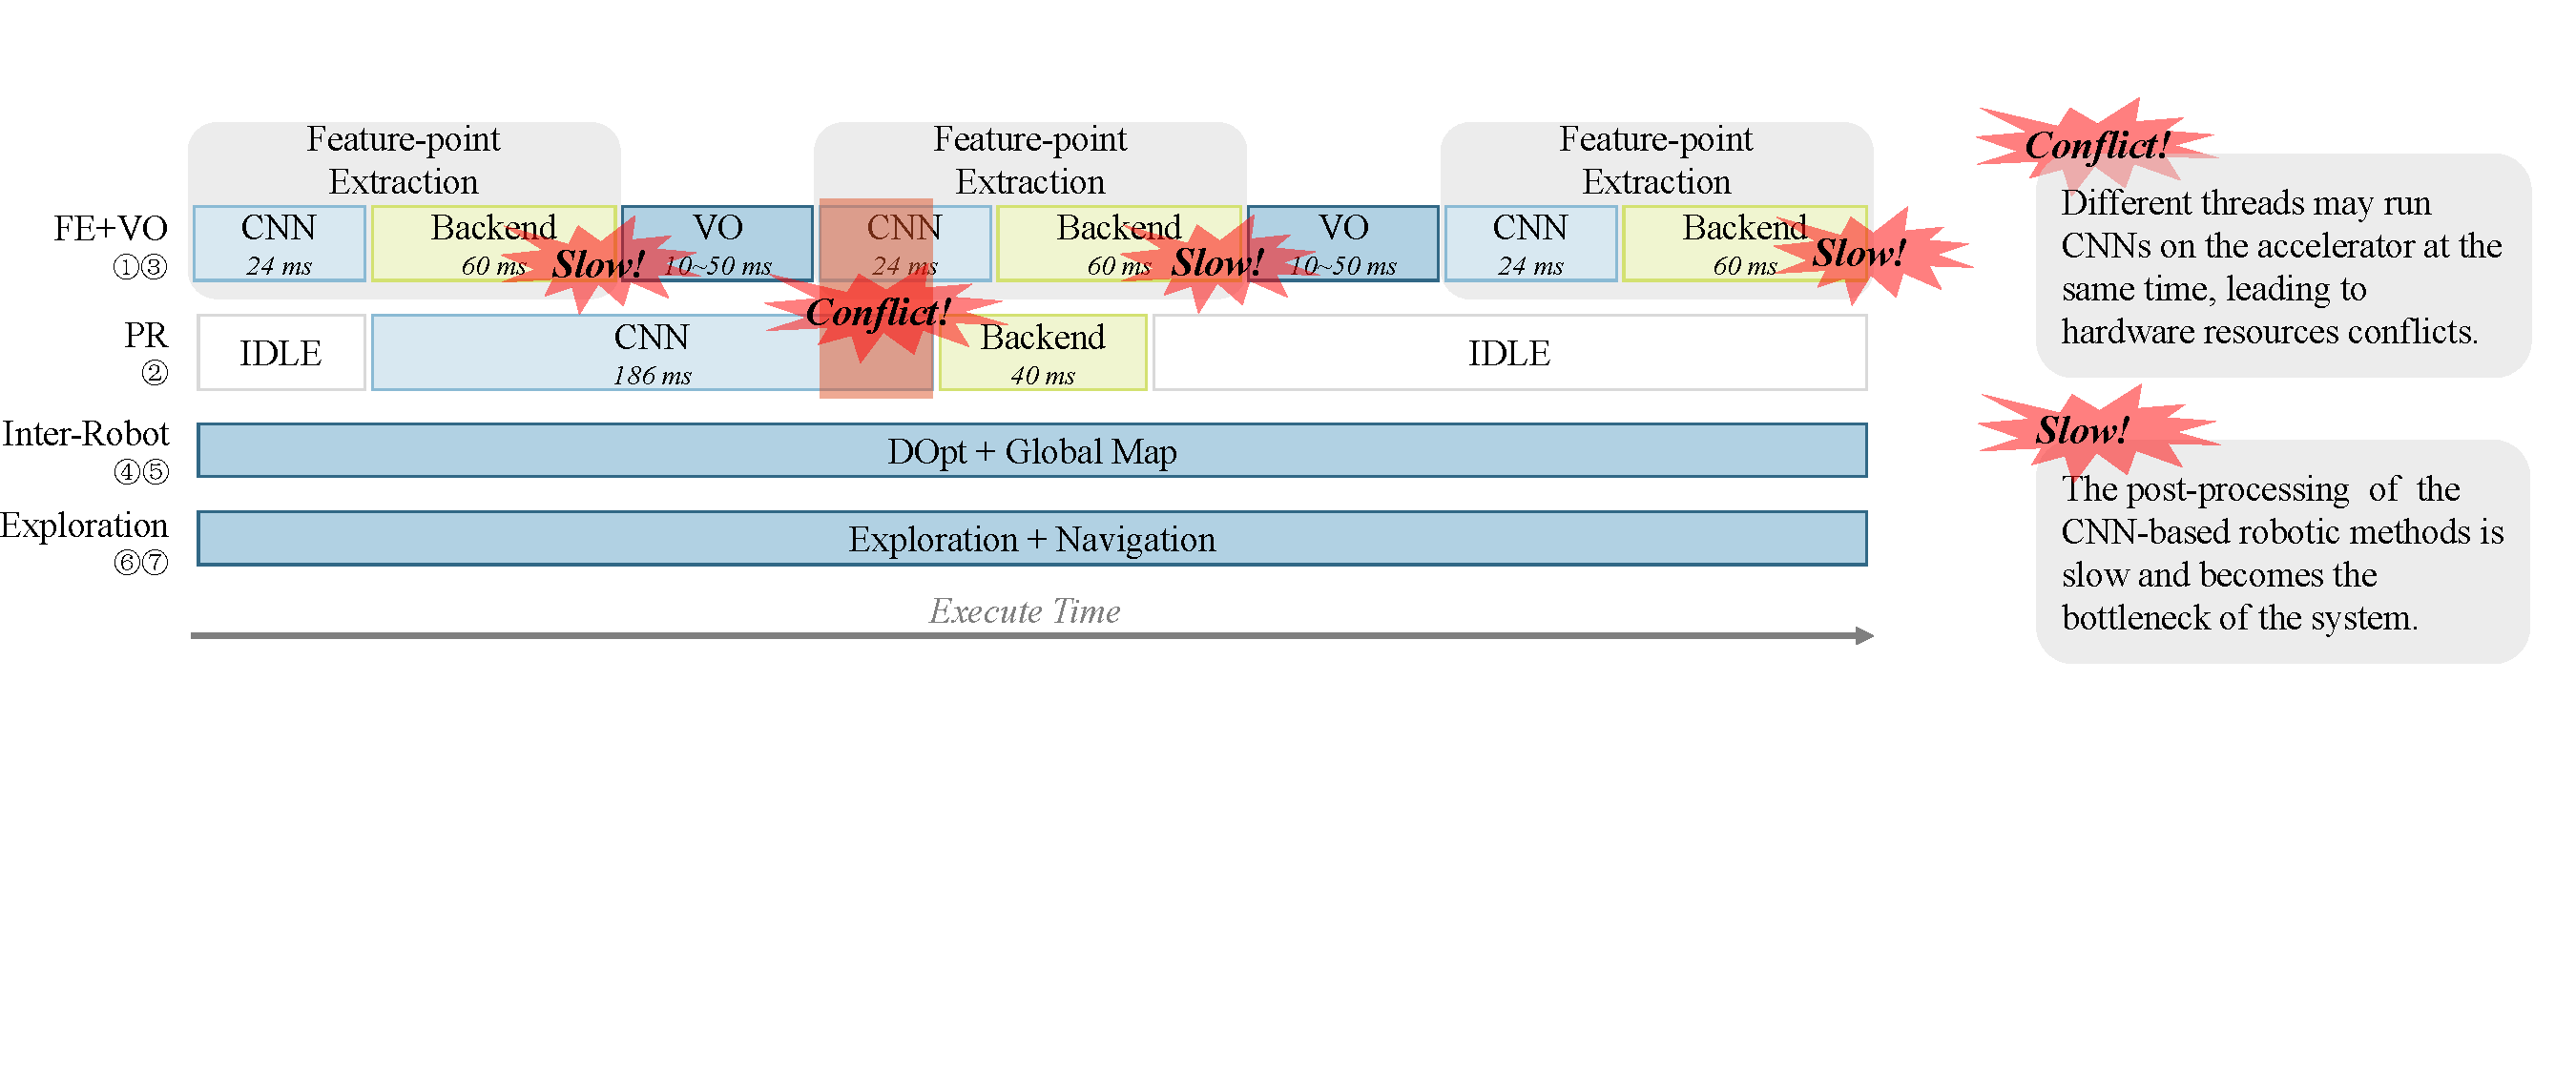
\includegraphics[width=0.99\textwidth]{fig/overalltime.pdf} 	
    \vspace{-2mm}
    \caption{
    The overall timeline of MR-Exploration. The FPGA accelerator is adapted in the feature-point extraction (FE) and place recognition (PR). The simultaneous occupancy of a single FPGA accelerator by these two software threads will lead to hardware resources conflicts. The post-processing of the visual odometry (VO) with feature-points on embedded CPU is time-costing and cannot meet the real-time requirements.
    }
	\label{fig:overalltime}
\end{figure*}

Recent works use CNN to extract feature-points  ~\cite{detone2018superpoint, simo2015discriminative, yi2016lift} and generate the place representation code  ~\cite{arandjelovic2016netvlad, radenovic2018fine}. 
Compared with the popular handcrafted extraction method, ORB ~\cite{Mur-Artal:2017281}, the CNN-based feature-point extraction method, SuperPoint  ~\cite{detone2018superpoint}, achieves 10\%-30\% higher matching accuracy.
The accuracy of the place recognition code based on another CNN-based method, GeM  ~\cite{radenovic2018fine}, is also about 20\% better than the handcrafted method, rootSIFT  ~\cite{jegou2014triang}.

% Thus, we adopt these CNN methods to realize Feature-point Extraction and  Place Recognition. 
Therefore, CNN is increasingly used in robotic systems. 
Besides these two components, more CNN-based methods, such as semantic segmentation  ~\cite{long2015fully} and object detection  ~\cite{ren2015faster}, can be introduced into robots to achieve better performance in the future. 

However, CNN is computation consuming. A single inference of the CNN-based SuperPoint feature-point extraction consumes 39G operations  ~\cite{detone2018superpoint}, while a single inference of the CNN-based GeM  place recognition consumes 192G operations  ~\cite{radenovic2018fine}.
Therefore, specific hardware architectures on FPGA  ~\cite{guo2017angel,yu2018instruction,li_high_2016,qiu2016going,lu_evaluating_2017} are designed to deploy CNN on the embedded system.
With the help of neural network quantization and on-chip data reuse, the speed of CNN accelerators on embedded FPGA achieves 3TOP/s  ~\cite{lu_evaluating_2017}, which can support the real-time execution of CNN-based feature-point extraction  ~\cite{detone2018superpoint}.
However, these CNN accelerators are designed and optimized to accelerate a single CNN. They cannot automatically schedule two or more tasks simultaneously. 
% Even if only FE and PR are implemented in CNN, the computational complexity reaches 1 TOP/s , which poses a challenge to the real-time performance of embedded systems.


% In recent years, FPGA is becoming a promising platform for algorithm acceleration. 

We do a simple profiling of MR-Exploration with the CNN accelerator. The CNN backbones of FE and  PR are executed on the FPGA accelerator (Angel-Eye ~\cite{guo2017angel}).
Other operations, including the post-processing of the CNN-based FE and PR, run on the PS side of Xilinx ZCU102 evaluation board ~\cite{zcu102}. The timeline of each component is illustrated in \Cref{fig:overalltime}. 
The threads of FE and PR may need to process CNN at the same time,  and the simultaneous requests of the accelerator will lead to hardware resources conflicts. For CNN accelerators, the inability of multi-task makes it difficult for researchers in robotics to use embedded FPGA.

In order to facilitate robotic researchers to run different CNN tasks simultaneously on the FPGA accelerator, the accelerator should support the following features:

\textbf{Multi-thread:} Different components in a robot are from different developers. Thus, the Robot Operating System (ROS)  ~\cite{quigley2009ros} is proposed as a middleware to fuse these independent components, and is widely used by robotic researchers. Each component is considered as an independent thread in ROS. Different threads should have independent access to the accelerator without knowing the status of others.


% A robot contains many components including perception, decision-making, and control. 
% The Robot Operating System (ROS)  ~\cite{quigley2009ros} is a popular middleware fusing different components from different developers. 
% In ROS, each module is considered as an independent thread on CPU. 
% Different threads should have easy access to the FPGA accelerator.

\textbf{Dynamic Scheduling:} The execution of CNN depends on other operations. For example, CNN-based FE (\textcircled{1} in \Cref{fig:maexp}) needs to be executed after the VO (\textcircled{3}) is completed. 
The VO is running on the CPU, and the execution time varies with the input data  ~\cite{mohanan2018survey} (10ms - 50ms in \Cref{fig:overalltime}). 
The accelerator cannot predict when to start a task. 
Therefore, the FPGA accelerator should be scheduled dynamically to support irregular task requests from the software.

\textbf{Scheduling by priority:} Different components have different priorities. The control and perception tasks usually have higher priorities, while the long-term decision and optimization have lower priorities  ~\cite{RamsauerKLM17}. The critical tasks, which are latency-sensitive,  need to be processed firstly on the accelerator.

The concept of interrupt  ~\cite{jen1974processor} is introduced to CPU in the 1960s. It enables the CPU to support dynamic multi-task scheduling according to priority to satisfy these three functions. Therefore, we introduce the concept of interrupt to the CNN accelerator in this paper to support multi-task on FPGA-based accelerators.

Besides the CNN backbones, the post-processing of the CNN-based methods, including normalization, softmax, rank, etc., are also computationally intensive. As illustrated in \Cref{fig:overalltime}, the execution time of post-processing for FE on embedded CPU (\textasciitilde 60ms) exceeds that of CNN backbone on the accelerator (\textasciitilde  30ms), and becomes the bottleneck of the system. 
As mentioned before, CNN is widely used in a variety of robot tasks.
The post-processing of these different tasks may become the new bottleneck of the system.
It is necessary to use FPGA to speed up post-processing, and a framework is also needed to organically integrate the CNN backbones and post-processing operations.

To address the above challenges, we propose an INterruptible CNN Accelerator for Multi-robot Exploration (INCAME) for rapid deployment of robot application on FPGA, with the following contributions:

\begin{itemize}
    % \begin{itemize}[leftmargin = 10 pt]
% \item We propose a CNN-based MR-Exploration framework based on FPGA. The hardware and software modules in INCAME is designed for ROS  ~\cite{quigley2009ros}, so that the modules can be easily used in other applications.
\item We propose a CNN-based MR-Exploration framework, INCAME. CNN-based methods for feature-point extraction (FE) and place recognition (PR) are accelerated with FPGA on the ROS platform ~\cite{quigley2009ros}. With the help of the unified interface in ROS, these CNN-based methods can be easily used by other developers in different applications.
\item We propose a \textbf{virtual-instruction-based} interrupt method to make the CNN accelerator support dynamic multi-task scheduling by priority. The method solves the hardware resources conflicts when accelerating different CNN tasks on ROS.
% \item We only needs to modify the instruction fetch module of the CNN accelerator in hardware to support interrupt. Thus, it is easy to be extended to different instruction-driven CNN accelerators.
\item We optimize the data flow of the post-processing operations. Hardware modules are also designed for the optimized post-processing. This software-hardware co-optimization assures the real-time performance of MR-Exploration .
\end{itemize}

The rest of this article is organized as follows: \Cref{sec:relate} introduces the related work. \Cref{sec:incame} introduces the INCAME framework with ROS. \Cref{sec:cnninterrupt} details the {virtual-instruction-based} interrupt. \Cref{sec:hardsoftcodesign} details the optimization of post-processing.  Experimental results and analysis are given in \Cref{sec:experiments}. \Cref{sec:conclusion} concludes this paper.